\documentclass[11pt,a4paper]{article}
\usepackage[textwidth=37em,vmargin=30mm]{geometry}
\usepackage{calc,xunicode,amsmath,amssymb,paralist,enumitem,tabu,booktabs,datetime2,xeCJK,xeCJKfntef,listings}
\usepackage{fancyhdr,tcolorbox,xcolor,graphicx,eso-pic,xltxtra,xelatexemoji}

\newcommand{\envyear}[0]{DATETHISYEAR}
\newcommand{\envdatestr}[0]{DATESTRING}
\newcommand{\envfinaldir}[0]{FINALDIR}

\usepackage[hidelinks]{hyperref}
\hypersetup{
    colorlinks=false,
    pdfpagemode=FullScreen,
    pdftitle={Web Digest - \envyear}
}

\setdefaultleftmargin{2em}{2em}{1em}{1em}{1em}{1em}

\usepackage{xeCJK,xeCJKfntef}
\newcommand{\myvphantom}[0]{\vphantom{QWERTYUIOPASDFGHJKLZXCVBNMqwertyuiopasdfghjklzxcvbnm1234567890ςρθδφγηξλζχψβμ\"A}}
\xeCJKsetup{PunctStyle=plain,RubberPunctSkip=false,CJKglue=\myvphantom\hskip 0pt plus 0.1em minus 0.05em,CJKecglue=\myvphantom\hskip 0.22em plus 200pt}
\XeTeXlinebreaklocale "zh"
\XeTeXlinebreakskip = 0pt


\setmainfont{Brygada 1918}
\setromanfont{Brygada 1918}
\setsansfont{IBM Plex Sans}
\setmonofont{JetBrains Mono NL}
\setCJKmainfont{Noto Serif CJK SC}
\setCJKromanfont{Noto Serif CJK SC}
\setCJKsansfont{Noto Sans CJK SC}
\setCJKmonofont{Noto Sans CJK SC}

\setlength{\parindent}{0pt}
\setlength{\parskip}{8pt}
\linespread{1.15}

\lstset{
	basicstyle=\ttfamily\footnotesize,
	numbersep=5pt,
	backgroundcolor=\color{black!5},
	showspaces=false,
	showstringspaces=false,
	showtabs=false,
	tabsize=2,
	captionpos=b,
	breaklines=true,
	breakatwhitespace=true,
	breakautoindent=true,
	linewidth=\textwidth
}






\newcommand{\coverpic}[2]{
    % argv: itemurl, authorname
    Cover photo by #2~~(\href{#1}{#1})
}
\newcommand{\makeheader}[0]{
    \begin{titlepage}
        % \newgeometry{hmargin=15mm,tmargin=21mm,bmargin=12mm}
        \begin{center}
            
            \rmfamily\scshape
            \fontspec{BaskervilleF}
            \fontspec{Old Standard}
            \fontsize{59pt}{70pt}\selectfont
            WEB\hfill DIGEST
            
            \vfill
            % \vskip 30pt
            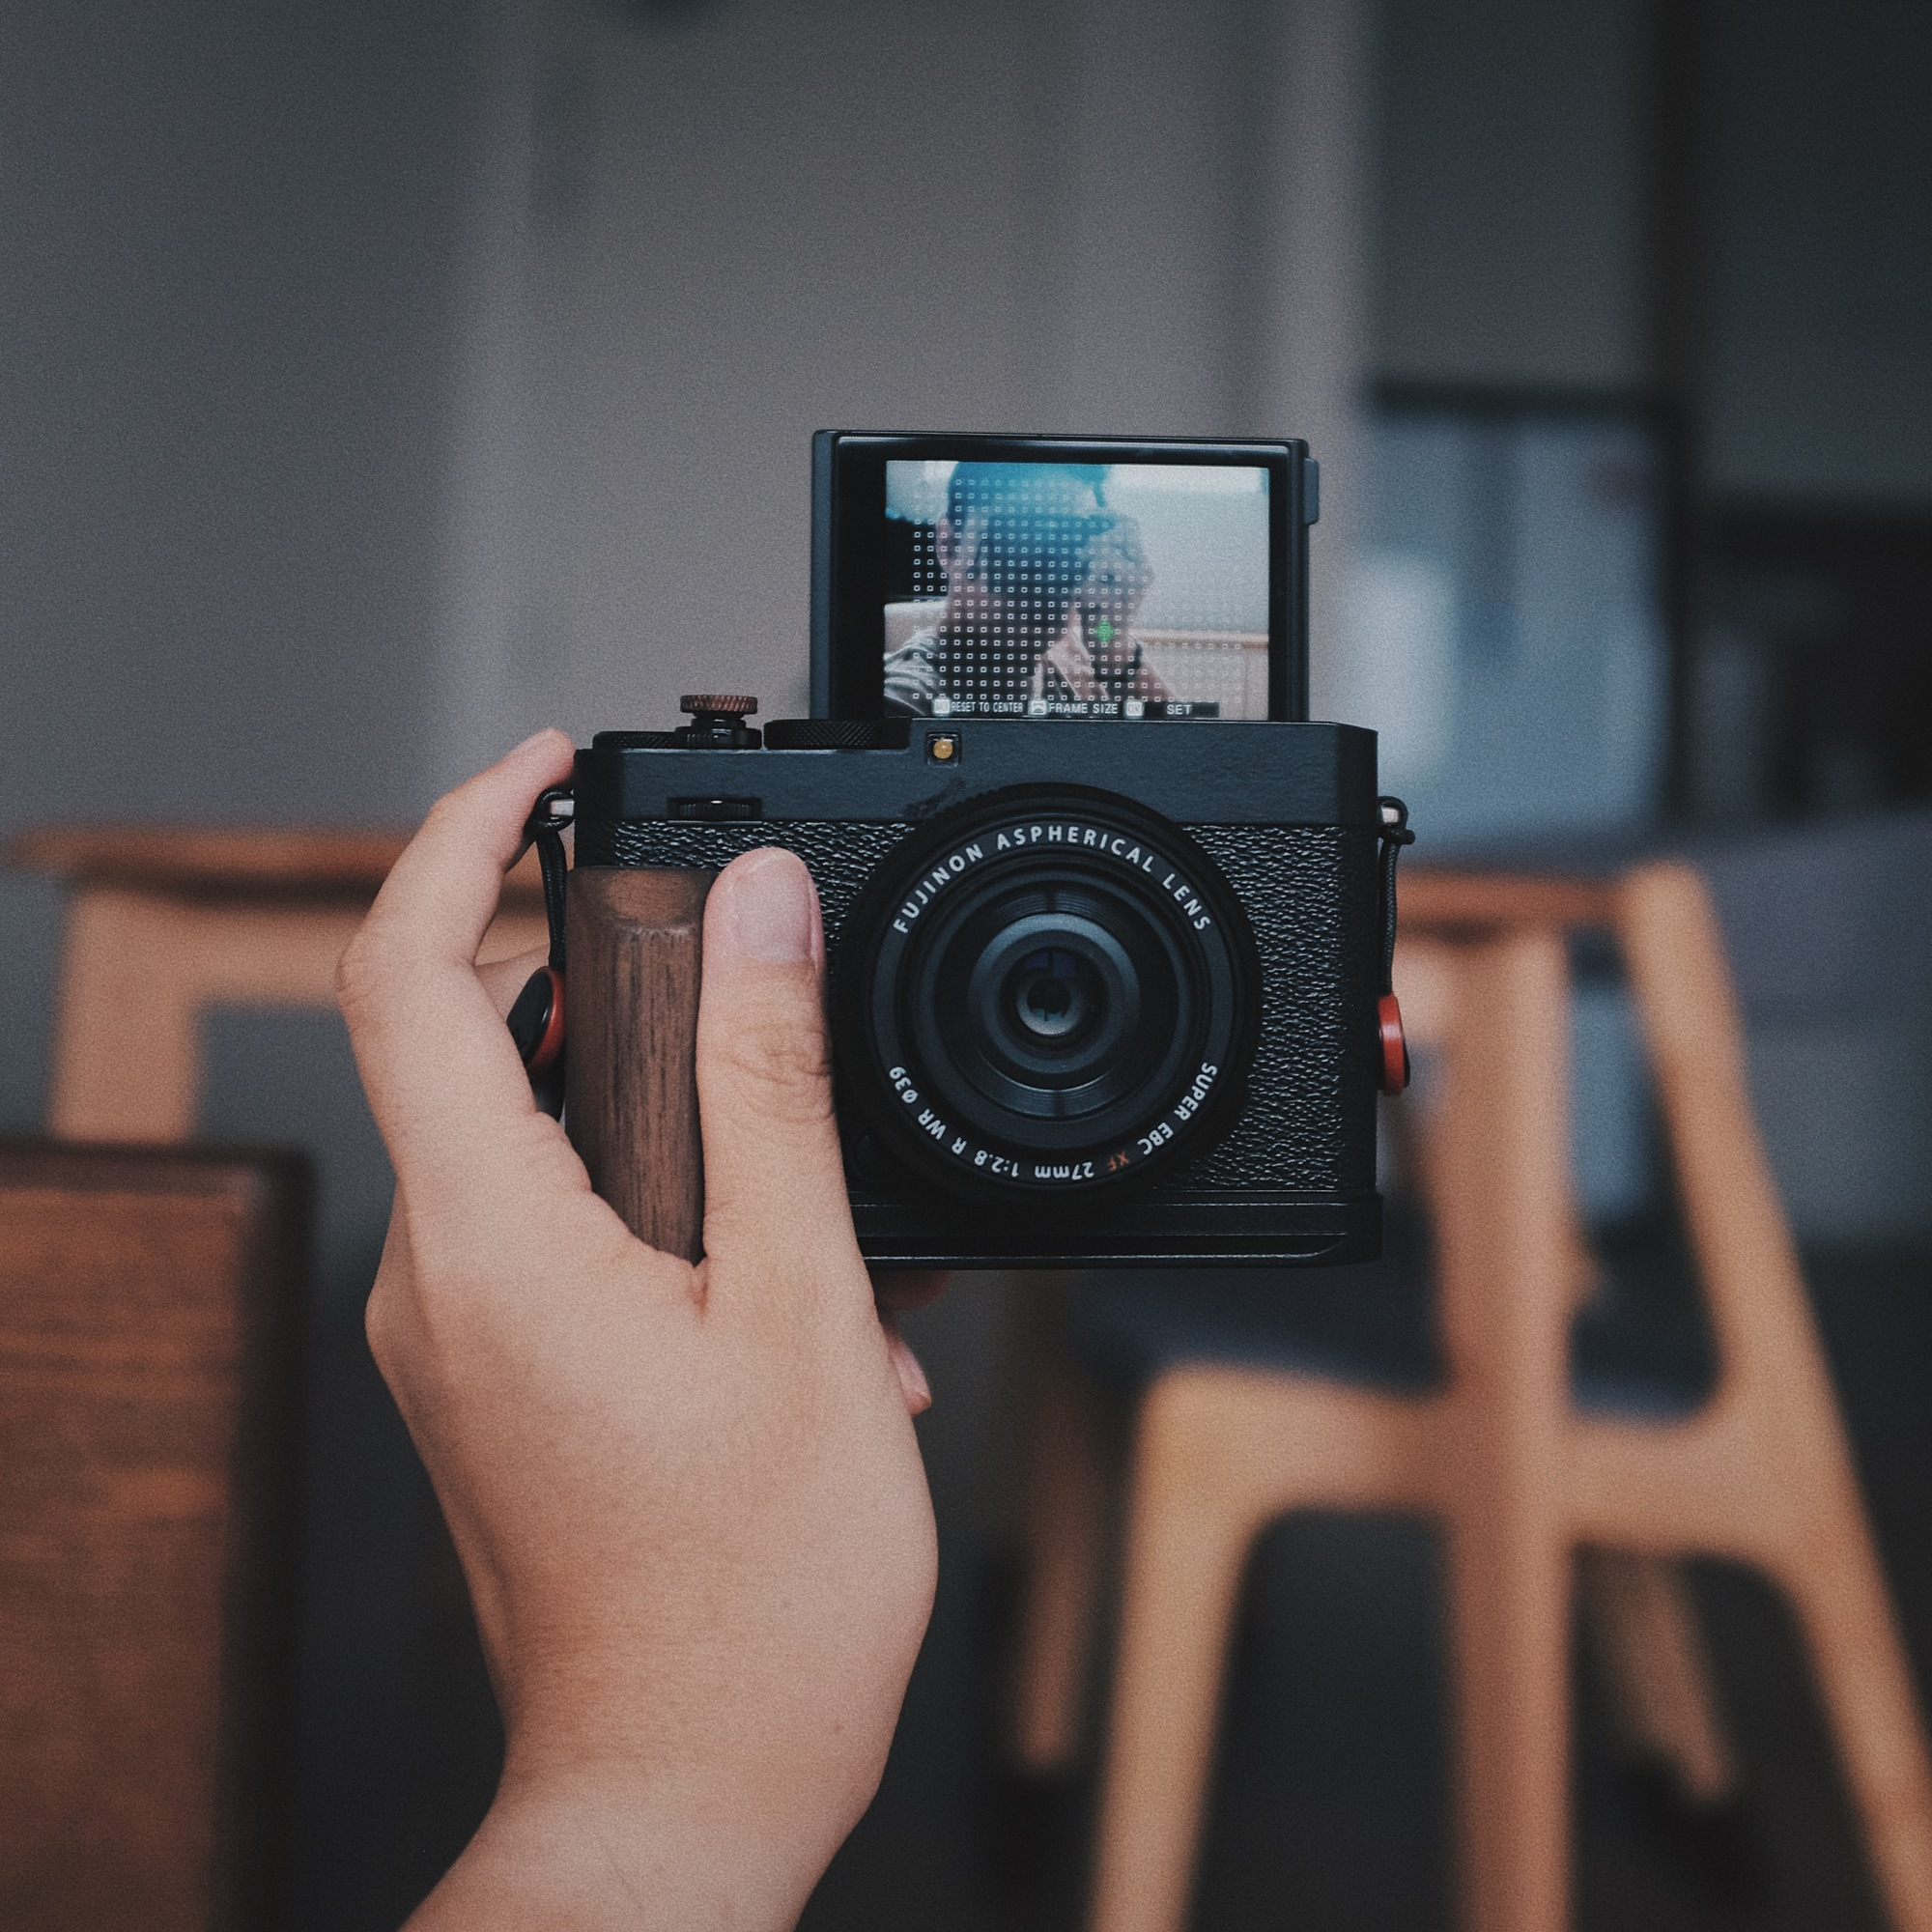
\includegraphics[width=\linewidth]{\envfinaldir/coverpic-prod.jpg}\par
            % \vskip 30pt
            \vfill

            \normalsize\rmfamily\scshape
            \copyright{} The Web Digest Project \hfill\large \envdatestr
        \end{center}
    \end{titlepage}
    % \restoregeometry
}
\newcommand{\simplehref}[1]{%
    \textcolor{blue!80!green}{\href{#1}{#1}}%
}
\renewcommand{\contentsname}{\center\Huge\sffamily\bfseries Contents\par\vskip 20pt}
\newcounter{ipartcounter}
\setcounter{ipartcounter}{0}
\newcommand{\ipart}[1]{
    % \vskip 20pt
    \clearpage
    \stepcounter{ipartcounter}
    \phantomsection
    \addcontentsline{toc}{chapter}{#1}
    % \begin{center}
    %     \Huge
    %     \sffamily\bfseries
    %     #1
    % \end{center}
    % \vskip 20pt plus 7pt
}
\newcounter{ichaptercounter}
\setcounter{ichaptercounter}{0}
\newcommand{\ichapter}[1]{
    % \vskip 20pt
    \clearpage
    \stepcounter{ichaptercounter}
    \phantomsection
    \addcontentsline{toc}{section}{\numberline{\arabic{ichaptercounter}}#1}
    \begin{center}
        \Huge
        \sffamily\bfseries
        #1
    \end{center}
    \vskip 20pt plus 7pt
}
\newcommand{\entrytitlefont}[1]{\subsection*{\raggedright\Large\sffamily\bfseries#1}}
\newcommand{\entryitemGeneric}[2]{
    % argv: title, url
    \parbox{\linewidth}{
        \entrytitlefont{#1}\par\vskip 5pt
        \footnotesize\ttfamily\mdseries
        \simplehref{#2}
    }\vskip 11pt plus 11pt minus 1pt
}
\newcommand{\entryitemGithub}[3]{
    % argv: title, url, desc
    \parbox{\linewidth}{
        \entrytitlefont{#1}\par\vskip 5pt
        \footnotesize\ttfamily\mdseries
        \simplehref{#2}\par\vskip 5pt
        \small\rmfamily\mdseries#3
    }\vskip 11pt plus 11pt minus 1pt
}
\newcommand{\entryitemAp}[3]{
    % argv: title, url, desc
    \parbox{\linewidth}{
        \entrytitlefont{#1}\par\vskip 5pt
        \footnotesize\ttfamily\mdseries
        \simplehref{#2}\par\vskip 5pt
        \small\rmfamily\mdseries#3
    }\vskip 11pt plus 11pt minus 1pt
}
\newcommand{\entryitemHackernews}[3]{
    % argv: title, hnurl, rawurl
    % \parbox{\linewidth}{
    %     \entrytitlefont{#1}\par\vskip 5pt
    %     \footnotesize\ttfamily\mdseries
    %     \simplehref{#3}\par
    %     \textcolor{black!50}{\href{#2}{#2}}
    % }\vskip 11pt plus 11pt minus 1pt
    \begin{minipage}{\linewidth}
            \entrytitlefont{#1}\par\vskip 5pt
            \footnotesize\ttfamily\mdseries
            \simplehref{#3}\par
            \textcolor{black!50}{\href{#2}{#2}}
    \end{minipage}\par\vskip 11pt plus 11pt minus 1pt
}







\begin{document}

\makeheader

\tableofcontents\clearpage




\ipart{Developers}
\ichapter{Hacker News}
\entryitemTwoLinks{What would it take to recreate Bell Labs?}{https://news.ycombinator.com/item?id=40998927}{https://www.construction-physics.com/p/what-would-it-take-to-recreate-bell}

\entryitemTwoLinks{USPS shared customer postal addresses with Meta, LinkedIn and Snap}{https://news.ycombinator.com/item?id=40998647}{https://techcrunch.com/2024/07/18/usps-shared-customer-postal-addresses-with-meta-linkedin-and-snap/}

\entryitemTwoLinks{Devzat – Chat over SSH, with some nice quality-of-life features}{https://news.ycombinator.com/item?id=40998158}{https://github.com/quackduck/devzat}

\entryitemTwoLinks{GPT-4o mini: advancing cost-efficient intelligence}{https://news.ycombinator.com/item?id=40997585}{https://openai.com/index/gpt-4o-mini-advancing-cost-efficient-intelligence/}

\entryitemTwoLinks{Polychromatic Pixels}{https://news.ycombinator.com/item?id=40997087}{https://compoundsemiconductor.net/article/119170/Polychromatic\_pixels}

\entryitemTwoLinks{Mistral NeMo}{https://news.ycombinator.com/item?id=40996058}{https://mistral.ai/news/mistral-nemo/}

\entryitemTwoLinks{Hash-based bisect debugging in compilers and runtimes}{https://news.ycombinator.com/item?id=40995982}{https://research.swtch.com/bisect}

\entryitemTwoLinks{Sparrows may be 'canary in the coal mine' for lead poisoning in children: study}{https://news.ycombinator.com/item?id=40995527}{https://www.abc.net.au/news/science/2024-07-18/sparrows-lead-poisoning-children-blood-levels-health-mining/104075894}

\entryitemTwoLinks{The Objects of Our Life (1983)}{https://news.ycombinator.com/item?id=40995515}{https://stevejobsarchive.com/exhibits/objects-of-our-life}

\entryitemTwoLinks{Ask HN: What's Prolog like in 2024?}{https://news.ycombinator.com/item?id=40994552}{https://news.ycombinator.com/item?id=40994552}

\entryitemTwoLinks{Collection of Dark Patterns and Unethical Design}{https://news.ycombinator.com/item?id=40993389}{https://hallofshame.design/collection/}

\entryitemTwoLinks{My daughter (7 years old) used HTML to make a website}{https://news.ycombinator.com/item?id=40992982}{https://naya.lol}

\entryitemTwoLinks{Amazon's Kindle Direct Publishing is a dystopian nightmare}{https://news.ycombinator.com/item?id=40992654}{https://news.ycombinator.com/item?id=40992654}

\entryitemTwoLinks{Americans' confidence in higher education has taken a nosedive}{https://news.ycombinator.com/item?id=40991894}{https://lithub.com/americans-confidence-in-higher-education-has-taken-a-nosedive/}

\entryitemTwoLinks{A RP2040 based DECstation 3000 emulator that can run DECWindows}{https://news.ycombinator.com/item?id=40991182}{https://github.com/rscott2049/DECstation2040}

\entryitemTwoLinks{Closed form arc length parametrization is impossible for quadratic Bézier curves}{https://news.ycombinator.com/item?id=40991075}{https://ninjakoa.la/curly\_curves/posts/quadratic\_bezier\_arc\_length\_parametrization/}

\entryitemTwoLinks{SAPwned: SAP AI vulnerabilities expose customers' cloud environments and privat}{https://news.ycombinator.com/item?id=40990768}{https://www.wiz.io/blog/sapwned-sap-ai-vulnerabilities-ai-security}

\entryitemTwoLinks{Show HN: SQLite Transaction Benchmarking Tool}{https://news.ycombinator.com/item?id=40990641}{https://github.com/seddonm1/sqlite-bench}

\entryitemTwoLinks{Show HN: Product Hunt for Music}{https://news.ycombinator.com/item?id=40989451}{https://tracklist.it/}

\entryitemTwoLinks{Little Languages (1986) [pdf]}{https://news.ycombinator.com/item?id=40989069}{https://staff.um.edu.mt/afra1/seminar/little-languages.pdf}\ichapter{Phoronix}
\entryitemGeneric{\hskip 0pt{}Freedreno Gallium3D Driver Now Enables The Snapdragon X1 Elite/Plus SoC's GPU}{https://www.phoronix.com/news/Freedreno-Snapdragon-X1-GPU}

\entryitemGeneric{\hskip 0pt{}Fedora 41 Proceeds With AMD SEV-SNP Virtualization Host Support For Confidential VMs}{https://www.phoronix.com/news/Fedora-41-Goes-AMD-SEV-SNP}

\entryitemGeneric{\hskip 0pt{}AWS Graviton4 96-Core Performance vs. AMD EPYC \& Intel Xeon CPUs}{https://www.phoronix.com/review/graviton4-96-core}

\entryitemGeneric{\hskip 0pt{}AMD RDNA4 "GFX12" Linux Driver Support Matures To Being Enabled By Default}{https://www.phoronix.com/news/AMD-RDNA4-Linux-Driver-Ready}

\entryitemGeneric{\hskip 0pt{}Sound Open Firmware 2.10 Brings Stable Support For Intel Arrow Lake \& Lunar Lake}{https://www.phoronix.com/news/Sound-Open-Firmware-2.10}

\entryitemGeneric{\hskip 0pt{}EXT4 Has A Very Nice Performance Optimization For Linux 6.11}{https://www.phoronix.com/news/Linux-6.11-EXT4}

\entryitemGeneric{\hskip 0pt{}GCC On AArch64 Handles Rewriting "-march=native" To "-mcpu=native"}{https://www.phoronix.com/news/GCC-AArch64-march-native-mcpu}

\entryitemGeneric{\hskip 0pt{}Fedora 41 Looks To Ship Upcoming AMD ROCm 6.2 For Latest AI Capabilities}{https://www.phoronix.com/news/AMD-ROCm-6.2-Fedora-41}

\entryitemGeneric{\hskip 0pt{}XFS Real-Time Enables FITRIM Support With Linux 6.11}{https://www.phoronix.com/news/XFS-RT-FITRIM-Linux-6.11}\ichapter{Dribbble}
\entryitemGeneric{\hskip 0pt{}Space Pencil Art Print}{https://dribbble.com/shots/24526524}

\entryitemGeneric{\hskip 0pt{}Dave Matthews Band Mansfield, MA Poster}{https://dribbble.com/shots/24526236}

\entryitemGeneric{\hskip 0pt{}Colorama Color Kit - Atomic Age Edition}{https://dribbble.com/shots/24525587}

\entryitemGeneric{\hskip 0pt{}Ah-Ha}{https://dribbble.com/shots/24525995}

\entryitemGeneric{\hskip 0pt{}Olympic keepsakes}{https://dribbble.com/shots/24525280}

\entryitemGeneric{\hskip 0pt{}Stillwell Collective Logo System}{https://dribbble.com/shots/24445747}

\entryitemGeneric{\hskip 0pt{}Finger}{https://dribbble.com/shots/24524211}

\entryitemGeneric{\hskip 0pt{}Paradise Brew Werks Logo Design}{https://dribbble.com/shots/24526111}

\entryitemGeneric{\hskip 0pt{}Dragönsteel}{https://dribbble.com/shots/24519719}

\entryitemGeneric{\hskip 0pt{}Precious Metal 3}{https://dribbble.com/shots/24493609}

\entryitemGeneric{\hskip 0pt{}Dimensional Delivery}{https://dribbble.com/shots/24507540}

\entryitemGeneric{\hskip 0pt{}Forks Crosswalk Mural 3/3}{https://dribbble.com/shots/24494024}

\entryitemGeneric{\hskip 0pt{}Ready to go}{https://dribbble.com/shots/24507528}

\entryitemGeneric{\hskip 0pt{}2D Caracter to 3D}{https://dribbble.com/shots/24372489}

\entryitemGeneric{\hskip 0pt{}Laughlin Leather Co. Secondary Logo}{https://dribbble.com/shots/24450561}

\entryitemGeneric{\hskip 0pt{}Turning gravity into a mere suggestion}{https://dribbble.com/shots/24510153}

\entryitemGeneric{\hskip 0pt{}Casa Bella}{https://dribbble.com/shots/24511981}

\entryitemGeneric{\hskip 0pt{}corner}{https://dribbble.com/shots/24511281}

\entryitemGeneric{\hskip 0pt{}Cards For "Imaginarium" Board Game}{https://dribbble.com/shots/24491261}

\entryitemGeneric{\hskip 0pt{}Starbase Brewing}{https://dribbble.com/shots/24511406}

\entryitemGeneric{\hskip 0pt{}Paradise Brew Werks Branding}{https://dribbble.com/shots/24511663}

\entryitemGeneric{\hskip 0pt{}腐った}{https://dribbble.com/shots/24512544}

\entryitemGeneric{\hskip 0pt{}Landscape Collage Series Textures}{https://dribbble.com/shots/24500738}

\entryitemGeneric{\hskip 0pt{}Metal Gear Sahelanthropus}{https://dribbble.com/shots/24510101}


\ipart{Developers~~~~(zh-Hans)}
\ichapter{Solidot}
\entryitemGeneric{\hskip 0pt{}印度交易所价值约 2.3 亿美元的加密货币被盗}{https://www.solidot.org/story?sid=78737}

\entryitemGeneric{\hskip 0pt{}逾四成日本公司没有使用 AI 的计划}{https://www.solidot.org/story?sid=78736}

\entryitemGeneric{\hskip 0pt{}狗和宠物猪能对人类哭泣和哼哼声做出反应}{https://www.solidot.org/story?sid=78735}

\entryitemGeneric{\hskip 0pt{}Cloudflare 报告 6.8\% 的互联网流量是恶意的}{https://www.solidot.org/story?sid=78734}

\entryitemGeneric{\hskip 0pt{}京都动画纵火案发生五周年}{https://www.solidot.org/story?sid=78733}

\entryitemGeneric{\hskip 0pt{}Meta 未来的多模 AI 模型将不提供给欧盟客户}{https://www.solidot.org/story?sid=78732}

\entryitemGeneric{\hskip 0pt{}英伟达全面转向开源 GPU 内核模块}{https://www.solidot.org/story?sid=78731}

\entryitemGeneric{\hskip 0pt{}调查显示 84\% 的 PC 用户不愿意为 AI 硬件支付溢价}{https://www.solidot.org/story?sid=78730}

\entryitemGeneric{\hskip 0pt{}GitLab 探索出售}{https://www.solidot.org/story?sid=78729}

\entryitemGeneric{\hskip 0pt{}Google Docs 加入 Markdown 支持}{https://www.solidot.org/story?sid=78728}

\entryitemGeneric{\hskip 0pt{}药物让动物寿命延长四分之一}{https://www.solidot.org/story?sid=78727}

\entryitemGeneric{\hskip 0pt{}为何三星电子的罢工主力是女性?}{https://www.solidot.org/story?sid=78726}

\entryitemGeneric{\hskip 0pt{}免疫疗法在彻底改变癌症治疗}{https://www.solidot.org/story?sid=78725}

\entryitemGeneric{\hskip 0pt{}OpenStreetMap 诞生二十周年}{https://www.solidot.org/story?sid=78724}

\entryitemGeneric{\hskip 0pt{}Craig Wright 在英国面临伪证调查}{https://www.solidot.org/story?sid=78723}

\entryitemGeneric{\hskip 0pt{}印度曾估值 220 亿美元的创业公司面临清算}{https://www.solidot.org/story?sid=78722}

\entryitemGeneric{\hskip 0pt{}美国资金退出中国风投市场}{https://www.solidot.org/story?sid=78721}

\entryitemGeneric{\hskip 0pt{}三年内有 22 名日漫盗版网站中国运营者受处罚}{https://www.solidot.org/story?sid=78720}

\entryitemGeneric{\hskip 0pt{}黑客声称从迪士尼公司窃取了 1.1 TB 数据}{https://www.solidot.org/story?sid=78719}

\entryitemGeneric{\hskip 0pt{}瑞典祖父母可通过照顾孙辈获得补贴}{https://www.solidot.org/story?sid=78718}\ichapter{V2EX}
\entryitemGeneric{\hskip 0pt{}[生活] 说走就走的旅行}{https://www.v2ex.com/t/1058439}

\entryitemGeneric{\hskip 0pt{}[宽带症候群] 网络卡顿原因排查}{https://www.v2ex.com/t/1058438}

\entryitemGeneric{\hskip 0pt{}[程序员] 发现自己的 commit 标题和内容越来越长了}{https://www.v2ex.com/t/1058436}

\entryitemGeneric{\hskip 0pt{}[OpenAI] 新模型 GPT-4o mini 来了!省留总结...}{https://www.v2ex.com/t/1058435}

\entryitemGeneric{\hskip 0pt{}[问与答] QQ 会员续费现在还有没有省钱的方法?}{https://www.v2ex.com/t/1058433}

\entryitemGeneric{\hskip 0pt{}[Android] 音乐名称格式混乱:周杰伦-晴天;晴天-周杰伦 请问哪个听歌软件能统一规范,方便搜索音乐}{https://www.v2ex.com/t/1058432}

\entryitemGeneric{\hskip 0pt{}[问与答] 有头像网站推荐吗?}{https://www.v2ex.com/t/1058431}

\entryitemGeneric{\hskip 0pt{}[Windows] 如何永久关闭联想拯救者的 logo 呼吸灯}{https://www.v2ex.com/t/1058430}

\entryitemGeneric{\hskip 0pt{}[职场话题] App 开发是不是完全没前途了?}{https://www.v2ex.com/t/1058429}

\entryitemGeneric{\hskip 0pt{}[macOS] 求推荐 Mac Claude 客户端}{https://www.v2ex.com/t/1058428}

\entryitemGeneric{\hskip 0pt{}[程序员] 2024 年,你还能明显感知到某个手机应用是 web 套壳吗?}{https://www.v2ex.com/t/1058427}

\entryitemGeneric{\hskip 0pt{}[奇思妙想] 开一个失业者的咖啡馆怎么样?}{https://www.v2ex.com/t/1058426}

\entryitemGeneric{\hskip 0pt{}[求职] [后端] 校招生入职某中厂后悔,求 v 友们捞一捞}{https://www.v2ex.com/t/1058425}

\entryitemGeneric{\hskip 0pt{}[奇思妙想] 一种安全且不容易遗忘的密码思路}{https://www.v2ex.com/t/1058424}

\entryitemGeneric{\hskip 0pt{}[问与答] 现在还有什么靠谱的笔记本软件吗?有 windows 和安卓,可云同步?}{https://www.v2ex.com/t/1058423}

\entryitemGeneric{\hskip 0pt{}[求职] [求职] [广州] 前端/11 年/React/Webpack/Typescript}{https://www.v2ex.com/t/1058421}

\entryitemGeneric{\hskip 0pt{}[程序员] 大家避坑, AI 出海群,接单互助,九旬\&卡卡}{https://www.v2ex.com/t/1058420}

\entryitemGeneric{\hskip 0pt{}[OpenAI] 有没有使用 gptapi.us 的?为啥 dall-e-3 没法用了}{https://www.v2ex.com/t/1058419}

\entryitemGeneric{\hskip 0pt{}[酷工作] 招聘贴 - 蚂蚁集团大数据部招后端 Java 开发 P6-P7}{https://www.v2ex.com/t/1058418}

\entryitemGeneric{\hskip 0pt{}[分享创造] 电子洁癖友好型之 iOS 纯快捷指令记账}{https://www.v2ex.com/t/1058416}

\entryitemGeneric{\hskip 0pt{}[问与答] 千兆宽带满速下载,光猫就死机是什么鬼?}{https://www.v2ex.com/t/1058415}

\entryitemGeneric{\hskip 0pt{}[问与答] 国内亚马逊购物途径}{https://www.v2ex.com/t/1058413}

\entryitemGeneric{\hskip 0pt{}[健康] 明天和意外,你永远不知道哪个会先来}{https://www.v2ex.com/t/1058412}

\entryitemGeneric{\hskip 0pt{}[问与答] 外区的 Amazon Prime 要怎么开通,网上找不到具体教程}{https://www.v2ex.com/t/1058411}

\entryitemGeneric{\hskip 0pt{}[问与答] 很迷茫,不知道如何改变现状}{https://www.v2ex.com/t/1058410}

\entryitemGeneric{\hskip 0pt{}[酷工作] 比特鹰(Web3 龙头企业)招收各岗位人才}{https://www.v2ex.com/t/1058407}

\entryitemGeneric{\hskip 0pt{}[微信] 有没有靠谱的导出微信聊天记录的方法?}{https://www.v2ex.com/t/1058406}

\entryitemGeneric{\hskip 0pt{}[宽带症候群] 如果家宽用 IPv6,域名是怎么对应的?}{https://www.v2ex.com/t/1058404}

\entryitemGeneric{\hskip 0pt{}[程序员] 请问一下各位大佬,最近想买一台服务器托管到机房去,有什么必须要注意的事项吗?}{https://www.v2ex.com/t/1058403}

\entryitemGeneric{\hskip 0pt{}[问与答] 请教日本的程序员加班情况,不胜感激!}{https://www.v2ex.com/t/1058402}

\entryitemGeneric{\hskip 0pt{}[微信] 微信分国内和海外版,那么贴吧和 QQ 有无区别对待}{https://www.v2ex.com/t/1058400}

\entryitemGeneric{\hskip 0pt{}[程序员] 基于 Dify Workflow 的文章智能分析实践}{https://www.v2ex.com/t/1058398}

\entryitemGeneric{\hskip 0pt{}[投资] 求教大佬,有哪些适合内地人用的美股券商?}{https://www.v2ex.com/t/1058397}

\entryitemGeneric{\hskip 0pt{}[随想] 无人机在消防和急救车等时间敏感领域上是否有较好的应用场景}{https://www.v2ex.com/t/1058395}

\entryitemGeneric{\hskip 0pt{}[反馈] v2EX 的 rss 订阅异常了}{https://www.v2ex.com/t/1058394}

\entryitemGeneric{\hskip 0pt{}[酷工作] [招人] 安卓 腾娱互动 武汉(12k-20k * 14)}{https://www.v2ex.com/t/1058392}

\entryitemGeneric{\hskip 0pt{}[旅行] 有谁去过常州恐龙园的,求教几个问题?}{https://www.v2ex.com/t/1058391}

\entryitemGeneric{\hskip 0pt{}[Surge] Surge for iOS 出两个车位!}{https://www.v2ex.com/t/1058390}

\entryitemGeneric{\hskip 0pt{}[OpenAI] 现在 ChatGPT 注册已经不需要手机号了吗?}{https://www.v2ex.com/t/1058389}

\entryitemGeneric{\hskip 0pt{}[服务器] 求一个服务器车位}{https://www.v2ex.com/t/1058387}

\entryitemGeneric{\hskip 0pt{}[Python] [新手求助] (可能是)websocket 的代理问题}{https://www.v2ex.com/t/1058386}

\entryitemGeneric{\hskip 0pt{}[分享发现] 一个人就能做的月入 10 万的项目}{https://www.v2ex.com/t/1058385}

\entryitemGeneric{\hskip 0pt{}[Windows] 基于 WLS2 的 docker desktop 无法将系统中的挂载目录,挂载到容器里}{https://www.v2ex.com/t/1058384}

\entryitemGeneric{\hskip 0pt{}[宽带症候群] baidu.com 不让 ping 了}{https://www.v2ex.com/t/1058383}

\entryitemGeneric{\hskip 0pt{}[ACG] 推荐一款二次元的 AI 图片生成产品}{https://www.v2ex.com/t/1058382}

\entryitemGeneric{\hskip 0pt{}[问与答] 有没有 不错的 劳动法 实践操作的书 推荐 用来防止恶意裁员}{https://www.v2ex.com/t/1058381}

\entryitemGeneric{\hskip 0pt{}[程序员] 独立开发者如何应对经济大萧条加业务无人问津组合拳?}{https://www.v2ex.com/t/1058380}

\entryitemGeneric{\hskip 0pt{}[宽带症候群] Speedtest app(国际版)中国移动的测速点一个都不剩了}{https://www.v2ex.com/t/1058379}

\entryitemGeneric{\hskip 0pt{}[职场话题] 我是否真的适合做程序员(精简版)}{https://www.v2ex.com/t/1058378}

\entryitemGeneric{\hskip 0pt{}[微信] 微信音频导出}{https://www.v2ex.com/t/1058377}


\ipart{Generic News}
\ichapter{AP News}
\entryitemWithDescription{\hskip 0pt{}Meet Crush, the rare orange lobster diverted from dinner plate to aquarium by Denver Broncos fans}{https://apnews.com/article/116b158ee773d84ce0211955f4b47f2a}{The Downtown Aquarium in Denver has a new resident --- a rare orange lobster that was rescued from a shipment of crustaceans delivered to a Red Lobster restaurant in Pueblo, Colorado. A long-term employee who is a dishwasher and head...}

\entryitemWithDescription{\hskip 0pt{}Lou Dobbs, conservative pundit and Fox Business host, dies at 78}{https://apnews.com/article/76c799df42c6b7d4912dece5d180b2de}{NEW YORK (AP) --- Lou Dobbs, the conservative political pundit and TV host who was a nightly presence on Fox Business Network for more than a decade, has died. He was 78. His death was announced Thursday in a post on his official X...}

\entryitemWithDescription{\hskip 0pt{}Shannen Doherty finalizes divorce hours before death}{https://apnews.com/article/0d9fbb475ae64fed1ccdc0a03eb69cf6}{LOS ANGELES (AP) --- Shannen Doherty finalized her split with husband, Kurt Iswarienko, just hours before her death at age 53, and she was granted a rare posthumous divorce two days later. Doherty, the star of ``Beverly Hills, 90210''...}

\entryitemWithDescription{\hskip 0pt{}Netflix's subscriber and earnings growth gather more momentum as password-sharing crackdown pays off}{https://apnews.com/article/d77c9a1f7ce29d1647354a7acf70a7ea}{Netflix's subscriber and earnings growth accelerated in its latest quarter as the video streaming service benefits from a crackdown on freeloading viewers, an expansion into advertising and an acclaimed programming lineup. The results...}

\entryitemWithDescription{\hskip 0pt{}Over 3 million steam cleaners are under recall because they can spew hot water and cause burns}{https://apnews.com/article/9a1d23b8f55cedf236e9d2a9d96ea2b5}{NEW YORK (AP) --- Some 3.3 million steam cleaners are being recalled across North America due to a burn hazard that has resulted in consumers reporting more than 150 injuries. Select models of Bissell-branded ``Steam Shot Handheld Steam...}

\entryitemWithDescription{\hskip 0pt{}After crash that killed 6 teens, NTSB chief says people underestimate marijuana's impact on drivers}{https://apnews.com/article/e25b14eca281d43efbdc6ee100573955}{DETROIT (AP) --- A horrific crash that killed six high school girls in Oklahoma two years ago has the head of the U.S. National Transportation Safety Board urging parents to warn teenagers about the risk of driving after using marijuana...}

\entryitemWithDescription{\hskip 0pt{}Passenger train derails in India, killing at least 2 passengers and injuring 20 others}{https://apnews.com/article/e98303b3f10a9751721791de1bb876c1}{LUCKNOW, India (AP) --- A passenger train derailed on Thursday in northern India, killing at least two passengers and injuring 20 others, a railroad official said. The cause of the accident is being investigated. Naveen Kumar, a state...}

\entryitemWithDescription{\hskip 0pt{}Historic utility AND high fashion. 80-year-old LL Bean staple finds a new audience as a trendy bag}{https://apnews.com/article/47a258dd282cdf3aee27878257b0418a}{FREEPORT, Maine (AP) --- L.L. Bean created it 80 years ago to haul heavy blocks of ice. Now it's a must-have summer fashion accessory. The simple, sturdy canvas bag called the Boat and Tote is having an extended moment 80 years after its...}

\entryitemWithDescription{\hskip 0pt{}Too soon for comedy? After attempted assassination of Trump, US politics feel anything but funny}{https://apnews.com/article/4235bd43f3750c95e0460d158996a0e5}{Political jokes: too soon? The answer from many quarters at midweek was a resounding yes, days after an assassination attempt against Republican former president Donald Trump rattled the nation over political violence that has been...}

\entryitemWithDescription{\hskip 0pt{}Caitlin Clark breaks WNBA's game assist record with 19 in Fever's loss to Wings}{https://apnews.com/article/cf9312845dfd08f6feab10b7da1dc410}{ARLINGTON, Texas (AP) --- Indiana rookie Caitlin Clark broke the WNBA record for assists in a game Wednesday night, finishing with 19 in the Fever's 101-93 loss to the Dallas Wings. ``I just try to set my teammates up for success,'' Clark...}

\entryitemWithDescription{\hskip 0pt{}Philadelphia Union midfielder Cavan Sullivan is the youngest ever in MLS. He's just 14 years old}{https://apnews.com/article/6e920552c38db70fd94bc94614f0e142}{CHESTER, Pa. (AP) --- Fourteen-year-old Philadelphia Union midfielder Cavan Sullivan became the youngest player in Major League Soccer history on Wednesday night --- and probably the youngest to play in any of the biggest professional...}

\entryitemWithDescription{\hskip 0pt{}Tons of dead fish cover major Sao Paulo river after alleged dumping of industrial waste}{https://apnews.com/article/5ecbe68b12e457cee242aebb5fdee509}{TANQUA, Brazil (AP) --- Several tons of fish have died along one of the main rivers in Sao Paulo state after an alleged illegal dumping of industrial waste from a sugar and ethanol plant, environmental authorities and prosecutors said on...}

\entryitemWithDescription{\hskip 0pt{}A meteor streaked across the NYC skyline before disintegrating over New Jersey}{https://apnews.com/article/52545d7d940dc1a63025ab447c3eaab2}{NEW YORK (AP) --- A meteor streaked across the New York City skyline before disintegrating over nearby New Jersey, according to NASA. William Cooke, the head of the space agency's Meteoroid Environments Office, said the fireball was first...}\ichapter{Reuters}
\entryitemWithDescription{\hskip 0pt{}Senate Republican Rubio defends Trump over Taiwan remarks}{https://www.reuters.com/world/us/senate-republican-rubio-defends-trump-over-taiwan-remarks-2024-07-18/}{Republican Senator Marco Rubio, who was a finalist to be Donald Trump\textquotesingle s running mate in the U.S. presidential campaign, said on Thursday he expected the U.S. would continue to support Taiwan under a Trump...}

\entryitemWithDescription{\hskip 0pt{}Air India Boeing plane bound to San Francisco lands in Russia}{https://www.reuters.com/world/air-india-boeing-plane-bound-san-francisco-lands-russia-2024-07-18/}{An Air India plane operating from Delhi to San Francisco made a precautionary landing in the Russian region of Siberia after the cockpit crew detected a potential issue in the cargo hold area, the Indian airline said on...}

\entryitemWithDescription{\hskip 0pt{}UK defence firms discuss boosting support for Ukraine with Zelenskiy}{https://www.reuters.com/business/aerospace-defense/uk-defence-firms-discuss-boosting-support-ukraine-with-zelenskiy-2024-07-18/}{Senior executives from British defence firms including BAE and Babcock met Ukrainian President Volodymyr Zelenskiy on Thursday to discuss the need to boost military support for the country in its conflict with...}

\entryitemWithDescription{\hskip 0pt{}Israeli strike kills field commander in elite Hezbollah unit, sources say}{https://www.reuters.com/world/middle-east/commander-hezbollahs-radwan-forces-killed-israeli-strike-south-lebanon-two-2024-07-18/}{A field commander in Hezbollah\textquotesingle s elite Radwan forces was killed in an Israeli strike on south Lebanon, two security sources said on Thursday, the latest senior member of the group to be killed in months of tit-for-tat...}

\entryitemWithDescription{\hskip 0pt{}French lawmakers re-elect Macron-ally Braun-Pivet as speaker in blow to left}{https://www.reuters.com/world/europe/french-lawmakers-re-elect-macron-ally-braun-pivet-speaker-blow-left-2024-07-18/}{Lawmakers in France\textquotesingle s National Assembly on Thursday handed centrist politician Yeael Braun-Pivet, a loyal ally of President Emmanuel Macron, a second term as speaker in a tight win over the candidate from the...}

\entryitemWithDescription{\hskip 0pt{}Chile to speed up construction of maximum security prison to fight organized crime}{https://www.reuters.com/world/americas/chile-speed-up-construction-maximum-security-prison-fight-organized-crime-2024-07-18/}{Chile will speed up construction of a new maximum security prison in the region that encompasses the capital city of Santiago to help fight organized crime, President Gabriel Boric announced on...}

\entryitemWithDescription{\hskip 0pt{}Attacker injures a police officer in central Paris, minister says}{https://www.reuters.com/world/europe/attacker-injures-one-police-officer-central-paris-attack-minister-2024-07-18/}{A police officer was critically injured in a stabbing attack in Paris\textquotesingle{} Champs Elysees shopping district on Thursday after a security guard at a boutique called police after spotting a man who appeared to be carrying a...}

\entryitemWithDescription{\hskip 0pt{}Biden continues to work amid 'mild' COVID symptoms, his doctor says}{https://www.reuters.com/world/us/biden-continues-work-amid-mild-covid-symptoms-his-doctor-says-2024-07-18/}{U.S. President Joe Biden is continuing to conduct official business while experiencing mild upper respiratory symptoms associated with his COVID diagnosis, his doctor said on Thursday, adding that the president\textquotesingle s vital...}

\entryitemWithDescription{\hskip 0pt{}France's Macron hopeful of addressing migration problems with British PM Starmer}{https://www.reuters.com/world/europe/frances-macron-hopeful-addressing-migration-problems-with-british-pm-starmer-2024-07-18/}{French President Emmanuel Macron said he was hopeful he would be able to work towards solutions for improving the situation linked to migration from France towards Britain in talks with British Prime Minister Keir Starmer on...}

\entryitemWithDescription{\hskip 0pt{}South Africa leader pledges to revive economy, include the poor}{https://www.reuters.com/world/africa/south-africas-new-government-prioritise-inclusive-economic-growth-ramaphosa-2024-07-18/}{President Cyril Ramaphosa pledged on Thursday to revive South Africa\textquotesingle s flagging economy and extend prosperity to the many left out of it, by resuscitating factories and farms, building roads and seizing the opportunities...}

\entryitemWithDescription{\hskip 0pt{}US to give another \$203 million in humanitarian aid for Sudanese}{https://www.reuters.com/world/us-give-another-203-million-humanitarian-aid-sudanese-2024-07-18/}{The United States will give an extra \$203 million to help millions of civilians affected by the war in Sudan, U.S. Ambassador to the United Nations Linda Thomas-Greenfield said on Thursday, calling on other nations to step up their...}

\entryitemWithDescription{\hskip 0pt{}Russia says 'let's be realistic' about Trump plan to end Ukraine war}{https://www.reuters.com/world/europe/russia-says-it-wont-accept-ultimatum-type-invitations-second-ukraine-peace-2024-07-18/}{Russia said on Thursday that Donald Trump\textquotesingle s assertion he could quickly end the Ukraine war should be viewed realistically, given that he had promised a Middle East peace breakthrough but failed to achieve it during his...}

\entryitemWithDescription{\hskip 0pt{}Russia says it may deploy nuclear missiles in response to US weapons in Germany}{https://www.reuters.com/world/russia-says-it-may-deploy-nuclear-missiles-response-us-weapons-germany-2024-07-18/}{Russia does not rule out new deployments of nuclear missiles in response to the planned U.S. stationing of long-range conventional weapons in Germany, Deputy Foreign Minister Sergei Ryabkov was quoted as saying on...}\ichapter{联合早报}
\entryitemWithDescription{美國前国安顾问建议台湾将国防开支提升到GDP 5\%}{https://www.zaobao.com/news/china/story20240718-4298225}{美国前总统特朗普点名台湾应向美国支付保护费后,特朗普政府时期的前国安顾问奥布莱恩说,面对中国大陆的潜在侵犯,台湾需要考虑将国防开支提升到至少本地生产总值( GDP)的5\%,以跟上大陆的发展步伐……}

\entryitemWithDescription{港消委会就农夫山泉测试样本归类出现落差致歉}{https://www.zaobao.com/news/china/story20240718-4297867}{香港消费者委员会日前点名中国大陆著名瓶装水品牌农夫山泉的饮用天然水溴酸盐含量达欧盟上限,遭该公司发律师函与要求道歉,港消委会随后称有关产品可安全饮用,又就是次测试样本归类有误致歉。事件引起陆港两地网民对大陆企业行为有无``霸凌''的热议……}

\entryitemWithDescription{中美舆论围绕中国游泳队兴奋剂风波隔空交锋}{https://www.zaobao.com/news/china/story20240718-4297908}{(北京/洛桑综合讯)巴黎奥运会下周即将开赛,中美舆论围绕中国游泳队兴奋剂风波隔空交锋。中国舆论称中国选手接受兴奋剂检测最为严格,美国舆论关注巴黎奥运会可能蒙上兴奋剂阴影。 中国国家游泳队营养师于良星期四(7月18日)在微博发文称,中国游泳队抵达法国的10天里,31名运动员除了训练、倒时差,还累计被国际兴奋剂检测机构(ITA)查了接近200人次,平均每天接近20人次,每人平均被查五至七次……}

\entryitemWithDescription{香港记者协会新任主席被《华尔街日报》解雇}{https://www.zaobao.com/news/china/story20240718-4296320}{(香港综合讯)新任香港记者协会主席郑嘉如称,因拒绝雇主《华尔街日报》要求其退出记协选举而被辞退。这是该报将亚洲总部从香港迁走后,再次在港掀起风波。 郑嘉如星期三(7月17日)在社交媒体平台X(原推特)发表声明,称《华尔街日报》以``架构重组''为由将她的职位裁撤。但郑嘉如认为,真正的原因是报社曾施压要她不要参选香港记协主席,并辞任理事一职,被她拒绝了……}

\entryitemWithDescription{四川自贡市百货大楼发生火灾 16人遇难}{https://www.zaobao.com/news/china/story20240718-4297534}{中国四川省自贡市九鼎百货大楼星期三发生火灾,消防救援车在火灾现场开展灭火和救援工作,救援工作到星期四凌晨3时结束。(中新社) 四川省自贡市的九鼎百货大楼星期三发生火灾,现场冒出大量浓烟。(法新社) (成都综合讯)中国四川省自贡市一家百货大楼星期三发生火灾,造成16人遇难。经初步调查,此次火灾由施工作业引发,相关责任人已被警方控制……}

\entryitemWithDescription{陈婧:楼市没有天气热}{https://www.zaobao.com/news/china/story20240718-4288625}{5月底上海放宽楼市限购政策初期,小区里的房产中介所久违地门庭若市。某天路过,房屋中介正劝说一名有意卖房的业主尽早挂牌,``趁现在市场回暖赶紧脱手,一个月后热度就又降了。'' 果然,进入7月后上海二手房交易量直线滑落。官方数据显示,7月前两周,二手房网签成交量9305套,比6月同期减少17%,没有一天网签成交量超过1000套……}

\entryitemWithDescription{港媒:中国27院士候选人因 ``打招呼'' 被永久取消资格}{https://www.zaobao.com/news/china/story20240717-4288285}{(北京综合讯)中国进一步规范科学院和工程院院士退出机制之后,据香港媒体报道,有27名院士候选人涉及``打招呼''而被永久取消参选资格。 中国人民网教育频道上星期五(7月12日)报道,在6月下旬举行的中国科学院第21次院士大会和中国工程院第17次院士大会,分别对院士章程进行了修订,进一步明确了两院院士的增选机制和退出机制……}

\entryitemWithDescription{特稿:江西企业实行``一带一路''战略调整 推动经济``外循环''}{https://www.zaobao.com/news/china/story20240717-3966505}{江铃新能源公司市面上售卖四款电动车车型,包括价格从约5万元人民币(9234万新元)起跳的微型车EV3。公司打算加强与全球经销商合作,将汽车销售到海外。(林煇智摄) 江西中煤建设集团(简称中煤集团)在南昌设有一个``一带一路''特色商品体验中心。这个名为``万国汇''的展厅,汇集了来自世界各地的食品,包括智利红酒、哈萨克斯坦骆驼奶粉、泰国茉莉香米、埃塞俄比亚咖啡等……}

\entryitemWithDescription{在野党团推动立法院解除赴陆禁团令 民进党团指决议抵触宪法因而无效}{https://www.zaobao.com/news/china/story20240717-4287907}{(台北综合讯)台湾立法院星期二通过解除限制民众组团赴中国大陆观光的决议,台湾政府大陆委员会表示尊重,但称将视台海两岸互动情况滚动检讨现行政策。 综合《联合报》和《台湾时报》报道,今年2月台湾交通部观光署发布赴陆禁团令,禁止民众组团赴大陆旅游,原定今年6月起暂停出团,后续放宽6月后已成团的旅客仍可出团,但旅游业者不得招揽新旅客……}

\entryitemWithDescription{中国暂停与美国商谈举行新一轮军控磋商}{https://www.zaobao.com/news/china/story20240717-4287695}{(北京综合讯)为了反制美国持续对台湾出售军备,中国外交部星期三宣布,暂停与美国商谈举行新一轮军控与防扩散磋商。 中国外交部发言人林剑星期三(7月17日)在例行记者会上称,一段时间以来,美国无视中国的坚决反对和反复交涉,持续对台军售,采取一系列严重损害中国的核心利益,破坏双方政治互信的消极举动,严重破坏双方继续进行军控磋商的政治气氛……}

\entryitemWithDescription{特朗普称台湾应向美国付军费 台行政院长:愿承担更多责任}{https://www.zaobao.com/news/china/story20240717-4286879}{预计星期四(7月18日)公布第二季度财报的台积电尚未就特朗普言论作出回应。图为7月16日的台积电新竹厂外观。(彭博社) (纽约/台北综合讯)美国前总统特朗普接受美国媒体采访时点名台湾应向美国支付军费,并指台湾夺走美国晶片业务,台积电股票星期三(7月17日)应声跌逾2\%,台湾行政院院长卓荣泰则称,台海的和平稳定是台湾、美国共同的责任和目标,台湾愿意承担更多的责任……}

\entryitemWithDescription{中国非在校青年失业率连续三个月下降}{https://www.zaobao.com/news/china/story20240717-4287249}{上海市民5月31日参加在该市中心举行的应届毕业生招聘会。(法新社) (北京综合讯)中国国家统计局最新数据显示,6月份全国非在校16岁至24岁青年失业率为13.2\%,较5月下降一个百分点,为连续三个月下降……}

\entryitemWithDescription{深圳失业金申领门槛提高 部分人遭追讨}{https://www.zaobao.com/news/china/story20240717-4286632}{(香港/华盛顿综合讯)中国经济重镇深圳市失业人口持续攀升之际,互联网流传消息指,该市失业金领取门槛提高,政府还向部分民众追讨已核发的失业金。 《南华早报》引述深圳市人力资源和社会保障局信息报道,该市今年第一季新增登记失业人数同比暴增40\%、环比增15\%,总劳动人口减少逾4万人。但这个数字不包括没有登记、或之前已登记过的失业人口。 失业人口上升意味着更多人有资格领取失业金……}

\entryitemWithDescription{中国商人郭文贵在美国被判欺诈罪}{https://www.zaobao.com/news/china/story20240717-4285905}{流亡美国的中国商人郭文贵被控诈骗超过10亿美元,图为郭文贵2017年4月在美国纽约接受媒体专访。(路透社档案照片) (纽约综合讯)流亡美国的中国商人郭文贵骗取投资者超过10亿美元,星期二(7月16日)在纽约被判欺诈罪,或将面临最高20年监禁。 综合路透社和彭博社报道,法庭星期二裁定郭文贵九项罪名成立,包括共谋敲诈勒索、证券欺诈以及共谋洗钱等。他将于11月19日被判刑……}

\entryitemWithDescription{戴庆成:香港年轻人为何躺平?}{https://www.zaobao.com/news/china/story20240717-4278076}{香港雇员再培训局一项调查显示,港青就业意欲偏低。一些斗志不强的香港年轻人则索性``躺平''。图为香港维多利亚港湾。(法新社) 近来香港楼价距离历史高位已经下跌了近三成,不过依然贵绝全球,大部分基层市民只能继续望``楼''兴叹。有调查显示,年轻人申请租住公屋蔚然成风,30岁以下拥有大专或以上学历申请者的比率在过去10年不断攀升,由33\%升至52\%……}

\entryitemWithDescription{深圳7月底开通首条自动驾驶公交车线路}{https://www.zaobao.com/news/china/story20240716-4279305}{图为深圳无人驾驶公交车。(互联网) (深圳/上海综合讯)继无人驾驶出租车(德士)在中国多个城市运行后,深圳市预计7月底正式开通首条自动驾驶公交车线路。 据深圳新闻网消息,深圳巴士集团计划于2024年内在深圳前海推广20台自动驾驶公交车,运营场景涵盖地铁站、商圈、居民住宅区、中央商务区、产业园区、文化旅游景区等,致力打造中国一线城市中心城区规模最大的自动驾驶公交车队……}

\entryitemWithDescription{哈马斯和法塔赫本月北京再会 分析:巴总统缺席和解可能性不大}{https://www.zaobao.com/news/china/story20240716-4279262}{以哈冲突持续了九个月,巴勒斯坦两股关系不睦的政治势力哈马斯和法塔赫,据报本月将在北京举行高层会晤,以结束巴勒斯坦内部分裂。中国外交部星期二(7月16日)并未否认这项消息。 受访学者分析,尽管哈马斯和法塔赫都提升此次赴北京会晤的代表层级,但领导法塔赫的巴勒斯坦总统阿巴斯预计缺席,因此与哈马斯正式和解的可能性不大……}

% \ipart{Hacker News}
% \entryitemTwoLinks{RealFill: Image completion using diffusion models}{https://news.ycombinator.com/item?id=37708292}{https://realfill.github.io/}

\entryitemTwoLinks{Homes ``unaffordable'' in 99\% of nation for average American}{https://news.ycombinator.com/item?id=37708109}{https://www.cbsnews.com/news/homes-for-sale-affordable-housing-prices/}

\entryitemTwoLinks{When CEOs Are Paid for Bad Performance (2005)}{https://news.ycombinator.com/item?id=37706876}{https://www.gsb.stanford.edu/insights/when-ceos-are-paid-bad-performance}

\entryitemTwoLinks{How a four-day workweek works, from the companies pulling it off}{https://news.ycombinator.com/item?id=37706596}{https://www.wsj.com/lifestyle/careers/how-a-4-day-workweek-actually-works-from-the-companies-pulling-it-off-1a5c0e2a}

\entryitemTwoLinks{Three Arrows Capital co-founder Zhu arrested in Singapore airport}{https://news.ycombinator.com/item?id=37705563}{https://techcrunch.com/2023/09/29/three-arrows-capital-co-founder-zhu-arrested-in-singapore-airport-sentenced-four-months-in-prison/}

\entryitemTwoLinks{Privacy washing: Google claims to support privacy while lobbying against it}{https://news.ycombinator.com/item?id=37705368}{https://proton.me/blog/google-lobbying}

\entryitemTwoLinks{Norway wants Facebook behavioral advertising banned across Europe}{https://news.ycombinator.com/item?id=37704859}{https://www.theregister.com/2023/09/29/norway\_facebook\_behavioral\_ads/}

\entryitemTwoLinks{Official U.S. government information about the Global Positioning System (GPS)}{https://news.ycombinator.com/item?id=37704593}{https://www.gps.gov/}

\entryitemTwoLinks{\$5k Google Jamboard dies in 2024–cloud-based apps will stop working, too}{https://news.ycombinator.com/item?id=37704537}{https://arstechnica.com/gadgets/2023/09/5000-google-jamboard-dies-in-2024-cloud-based-apps-will-stop-working-too/}

\entryitemTwoLinks{Encrypted Client Hello}{https://news.ycombinator.com/item?id=37703885}{https://blog.cloudflare.com/announcing-encrypted-client-hello/}

\entryitemTwoLinks{Senator Dianne Feinstein has died}{https://news.ycombinator.com/item?id=37703767}{https://www.bbc.com/news/world-us-canada-66963341}

\entryitemTwoLinks{Dianne Feinstein has died}{https://news.ycombinator.com/item?id=37703528}{https://www.nytimes.com/2023/09/29/us/politics/dianne-feinstein-dead-senate.html}

\entryitemTwoLinks{iPhone 15: users of Pro and Pro Max models complain of overheating issues}{https://news.ycombinator.com/item?id=37702846}{https://www.theguardian.com/technology/2023/sep/29/iphone-15-users-of-pro-and-pro-max-models-complain-of-overheating-issues}

\entryitemTwoLinks{Ask HN: Why isn't Phoenix/Elixir more mainstream?}{https://news.ycombinator.com/item?id=37702845}{https://news.ycombinator.com/item?id=37702845}

\entryitemTwoLinks{Everything authenticated by Microsoft is tainted}{https://news.ycombinator.com/item?id=37702095}{https://graz.social/@publicvoit/111147782761723981}

\entryitemTwoLinks{Leaked screenshot shows Amazon now tracking individual employee attendance}{https://news.ycombinator.com/item?id=37701222}{https://www.businessinsider.com/amazon-forced-rto-tracking-employee-office-attendance-2023-9}

\entryitemTwoLinks{Things Every Hacker Once Knew (2017)}{https://news.ycombinator.com/item?id=37701117}{http://www.catb.org/~esr/faqs/things-every-hacker-once-knew/}

\entryitemTwoLinks{Burning money on paid ads for a dev tool – what we've learned}{https://news.ycombinator.com/item?id=37700847}{https://posthog.com/blog/dev-marketing-paid-ads}

\entryitemTwoLinks{Richard Stallman reveals he has cancer in the GNU 40 Hacker Meeting talk [video]}{https://news.ycombinator.com/item?id=37699851}{https://audio-video.gnu.org/video/gnu40/rms-gnu40.webm}

\entryitemTwoLinks{Costco gold bars are selling out within hours}{https://news.ycombinator.com/item?id=37699396}{https://www.cnbc.com/2023/09/27/costco-is-selling-gold-bars-and-they-are-selling-out-within-a-few-hours.html}

% \ipart{V2EX}
% \entryitemGeneric{\hskip 0pt{}[问与答] 假如身边同事说以前拍过 A 片,你对他/她会是什么感觉?}{https://www.v2ex.com/t/945394}

\entryitemGeneric{\hskip 0pt{}[Apple] 纵观 618 手机推荐,好像 iphone15 的最大讨论是 C 口?}{https://www.v2ex.com/t/945393}

\entryitemGeneric{\hskip 0pt{}[问与答] 配一台 PVE 专用主机}{https://www.v2ex.com/t/945392}

\entryitemGeneric{\hskip 0pt{}[问与答] 请教一下,我这老古董的电脑配置,可以更新下显卡么?谢谢 V 友。}{https://www.v2ex.com/t/945391}

\entryitemGeneric{\hskip 0pt{}[程序员] 很多程序员确实会被后浪拍死在沙滩上}{https://www.v2ex.com/t/945390}

\entryitemGeneric{\hskip 0pt{}[推广] 手机版 ChatGPT,不需要魔法上网}{https://www.v2ex.com/t/945389}

\entryitemGeneric{\hskip 0pt{}[NAS] Nas 用作备份还是主存储}{https://www.v2ex.com/t/945387}

\entryitemGeneric{\hskip 0pt{}[问与答] virtctl 上传一个 iso 文件报错求助}{https://www.v2ex.com/t/945386}

\entryitemGeneric{\hskip 0pt{}[iDev] 看了微软的 documentation 才知道 macCatalyst 的预设 idiom 真的就是 .pad。}{https://www.v2ex.com/t/945385}

\entryitemGeneric{\hskip 0pt{}[程序员] 2 个适合做 AI 项目的域名}{https://www.v2ex.com/t/945384}

\entryitemGeneric{\hskip 0pt{}[Markdown] 贺 WWDC 😀,促销一下我的 App,时间 6/3~6/10,共 7 天,最低 6 折!}{https://www.v2ex.com/t/945383}

\entryitemGeneric{\hskip 0pt{}[OpenAI] depay 被 gpt 禁用了,大家有别的支付方式吗?}{https://www.v2ex.com/t/945382}

\entryitemGeneric{\hskip 0pt{}[分享发现] 去广告的油猴脚本里偷偷藏了个广告 dadiyouhui}{https://www.v2ex.com/t/945379}

\entryitemGeneric{\hskip 0pt{}[Flutter] 求助 flutter 代码 按钮提示音 问题}{https://www.v2ex.com/t/945377}

\entryitemGeneric{\hskip 0pt{}[生活] 失业设计师推广一下自创品牌香薰}{https://www.v2ex.com/t/945375}

\entryitemGeneric{\hskip 0pt{}[问与答] 美国 non tax resident  alien 个税 收入来自 paypal}{https://www.v2ex.com/t/945374}

\entryitemGeneric{\hskip 0pt{}[程序员] 计划写个全栈的浏览器插件开发教程,内容涉及 Web3, 前端,后端,浏览器开发,有没有感兴趣的!}{https://www.v2ex.com/t/945373}

\entryitemGeneric{\hskip 0pt{}[问与答] 我常常固执地沉浸在负面情绪中}{https://www.v2ex.com/t/945372}

\entryitemGeneric{\hskip 0pt{}[程序员] 程序员的悲哀是什么[转]}{https://www.v2ex.com/t/945371}

\entryitemGeneric{\hskip 0pt{}[北京] 谁有推荐配眼镜的地方}{https://www.v2ex.com/t/945366}

\entryitemGeneric{\hskip 0pt{}[问与答] Win10 自动安装管家}{https://www.v2ex.com/t/945365}

\entryitemGeneric{\hskip 0pt{}[iPhone] iPhone 第三方无线充电器推荐}{https://www.v2ex.com/t/945363}

\entryitemGeneric{\hskip 0pt{}[上海] 房东直租静安区二房无中介费}{https://www.v2ex.com/t/945362}

\entryitemGeneric{\hskip 0pt{}[问与答] s23u 港版}{https://www.v2ex.com/t/945361}

\entryitemGeneric{\hskip 0pt{}[硬件] 第一次攒机, NAS + HPC 求建议}{https://www.v2ex.com/t/945360}

\entryitemGeneric{\hskip 0pt{}[问与答] 打算在理想 L9 后排看奈飞,买了谷歌 TV,求推荐能装 CLASH 插件的 USB 无线 4G 网卡}{https://www.v2ex.com/t/945359}

\entryitemGeneric{\hskip 0pt{}[问与答] GitHub 改用户名,会对已有 repository 造成啥影响吗?}{https://www.v2ex.com/t/945357}

\entryitemGeneric{\hskip 0pt{}[深圳] 人在深圳,卖家电啦, TCL 家电,内购价,有需要购买家电的可以找我,提供贴心服务,优惠大大滴,全部都是成本价,不赚家人们一分钱,只为完成 kpi}{https://www.v2ex.com/t/945356}

\entryitemGeneric{\hskip 0pt{}[问与答] win10 睡眠唤醒之后,键盘无法用。}{https://www.v2ex.com/t/945355}

\entryitemGeneric{\hskip 0pt{}[问与答] 咨询一下大佬们,四个风扇的乔思伯 D41 Mesh 网孔版 白色,该怎么安排风道?}{https://www.v2ex.com/t/945354}

\entryitemGeneric{\hskip 0pt{}[奇思妙想] 在无 KVM 功能但有一线通的显示器上把它变成手动 KVM 模式是否可行?}{https://www.v2ex.com/t/945353}

\entryitemGeneric{\hskip 0pt{}[问与答] bilibili 电视 app 除了原生还有什么选择吗}{https://www.v2ex.com/t/945352}

\entryitemGeneric{\hskip 0pt{}[Apple] 总觉得 MBP 比 mac studio 用起来流畅的多。}{https://www.v2ex.com/t/945351}

\entryitemGeneric{\hskip 0pt{}[程序员] 大家觉得现在 CS Research 还有什么领域不卷}{https://www.v2ex.com/t/945350}

\entryitemGeneric{\hskip 0pt{}[Surge] [Surge for Mac 5 ] 160RMB/位}{https://www.v2ex.com/t/945349}

\entryitemGeneric{\hskip 0pt{}[生活] 查出了不能生育,心里郁闷}{https://www.v2ex.com/t/945348}

\entryitemGeneric{\hskip 0pt{}[分享创造] 面试工具 InterviewAI 在 ProductHunt 上发布啦}{https://www.v2ex.com/t/945347}

\entryitemGeneric{\hskip 0pt{}[Docker] docker run 成功, docker compose up 失败?}{https://www.v2ex.com/t/945345}

\entryitemGeneric{\hskip 0pt{}[分享发现] 看在 CPU 的面子上,多多入手红米 NOTE12 Turbo}{https://www.v2ex.com/t/945344}

\entryitemGeneric{\hskip 0pt{}[Amazon Web Services] AWS 的 cloudwatch 是必须使用的吗?}{https://www.v2ex.com/t/945343}

\entryitemGeneric{\hskip 0pt{}[问与答] 有没有卸载 Anaconda 不影响已经配置的环境切换到 Miniconda 的办法?}{https://www.v2ex.com/t/945341}

\entryitemGeneric{\hskip 0pt{}[分享创造] 低成本做个 ChatGPT 聊天机器人}{https://www.v2ex.com/t/945340}

\entryitemGeneric{\hskip 0pt{}[问与答] 海南的国企,海南征信,中科电海信院有没有好的建议}{https://www.v2ex.com/t/945338}

\entryitemGeneric{\hskip 0pt{}[生活] 如何处理收废品的大喇叭扰民?}{https://www.v2ex.com/t/945337}

\entryitemGeneric{\hskip 0pt{}[问与答] 二手车混动求推荐贬值超快的}{https://www.v2ex.com/t/945336}

\entryitemGeneric{\hskip 0pt{}[YubiKey] 收购两只 yubikey 5 nfc}{https://www.v2ex.com/t/945335}

\entryitemGeneric{\hskip 0pt{}[问与答] 除了豆瓣网,还有什么中文的图书、书评网吗?}{https://www.v2ex.com/t/945334}

\entryitemGeneric{\hskip 0pt{}[问与答] 高价求各种引流大佬}{https://www.v2ex.com/t/945332}

\entryitemGeneric{\hskip 0pt{}[OpenAI] 4.0api,claude 100kapi}{https://www.v2ex.com/t/945329}

\entryitemGeneric{\hskip 0pt{}[问与答] 求问 hw-v2-web-player-tracker.biliapi 是干什么的, clash 速率离奇达到 300MB/s}{https://www.v2ex.com/t/945326}

% \ipart{Solidot}
% \entryitemGeneric{\hskip 0pt{}科学家首次计算出恒星周围的含水量}{https://www.solidot.org/story?sid=77506}

\entryitemGeneric{\hskip 0pt{}印度要求发布模型需得到政府批准}{https://www.solidot.org/story?sid=77505}

\entryitemGeneric{\hskip 0pt{}防火墙泄漏跨国流量}{https://www.solidot.org/story?sid=77504}

\entryitemGeneric{\hskip 0pt{}中国盗版动漫网站主犯被判三年缓刑三年六个月}{https://www.solidot.org/story?sid=77503}

\entryitemGeneric{\hskip 0pt{}《ACM 通讯》正式拥抱开放获取}{https://www.solidot.org/story?sid=77502}

\entryitemGeneric{\hskip 0pt{}Linux 基金会的新项目得到了盖茨基金会的资助}{https://www.solidot.org/story?sid=77501}

\entryitemGeneric{\hskip 0pt{}Mozilla 的 Firefox 和谋智的火狐}{https://www.solidot.org/story?sid=77500}

\entryitemGeneric{\hskip 0pt{}两部星战电影准备开拍}{https://www.solidot.org/story?sid=77499}

\entryitemGeneric{\hskip 0pt{}全球人口的八分之一肥胖}{https://www.solidot.org/story?sid=77498}

\entryitemGeneric{\hskip 0pt{}Google 解雇了组建工会的 YouTube 合同工}{https://www.solidot.org/story?sid=77497}

\entryitemGeneric{\hskip 0pt{}座头鲸首次观察到同性性交}{https://www.solidot.org/story?sid=77496}

\entryitemGeneric{\hskip 0pt{}微软撤下导致``内存不足''错误的 Edge 更新}{https://www.solidot.org/story?sid=77495}

\entryitemGeneric{\hskip 0pt{}马斯克起诉 OpenAI 和 Sam Altman``违反合同''}{https://www.solidot.org/story?sid=77494}

\entryitemGeneric{\hskip 0pt{}美国疾控中心称 COVID-19 越来越像流感}{https://www.solidot.org/story?sid=77493}

\entryitemGeneric{\hskip 0pt{}BCUninstaller:轻松卸载你不想要的应用}{https://www.solidot.org/story?sid=77492}

% \ipart{Phoronix}
% \entryitemGeneric{\hskip 0pt{}AlmaLinux 10.1 Will Support The Btrfs File-System}{https://www.phoronix.com/news/AlmaLinux-10.1-Btrfs-Plans}

\entryitemGeneric{\hskip 0pt{}Valkey 9.0 Released With Ability To Achieve One Billion Requests / Second}{https://www.phoronix.com/news/Valkey-9.0-Released}

\entryitemGeneric{\hskip 0pt{}Intel Nova Lake To Feature 6th Gen NPU}{https://www.phoronix.com/news/Intel-Nova-Lake-6th-Gen-NPU}

\entryitemGeneric{\hskip 0pt{}Revisiting The SNC3 vs. HEX Mode Performance With Intel Xeon 6 Granite Rapids}{https://www.phoronix.com/review/intel-xeon-snc3-hex-benchmarks}

\entryitemGeneric{\hskip 0pt{}TARmageddon Strikes: High Profile Security Vulnerability In Popular Rust Library}{https://www.phoronix.com/news/Rust-TARmageddon}

\entryitemGeneric{\hskip 0pt{}More Kernel Graphics Driver \& Accelerator/NPU Driver Updates Ready For Linux 6.19}{https://www.phoronix.com/news/Linux-6.19-DRM-Misc-Next-2}

\entryitemGeneric{\hskip 0pt{}AMD PMF Linux Driver Working On AMD SystemDeck Support}{https://www.phoronix.com/news/AMD-PMF-Linux-SystemDeck}

\entryitemGeneric{\hskip 0pt{}Linux 6.19 Will Add Support For The Logitech G13 Keypad - 17 Years After Hardware Debut}{https://www.phoronix.com/news/Logitech-G13-For-Linux-6.19}

\entryitemGeneric{\hskip 0pt{}Blender 5.1 Aiming For Vulkan By Default, More Improvements Coming}{https://www.phoronix.com/news/Blender-5.1-Vulkan-Default}

% \ipart{联合早报}
% \entryitemWithDescription{杨丹旭:中国股民能否过个安心年?}{https://www.zaobao.com/news/china/story20240207-1466809}{``人生不仅仅只有股市,还有父母、爱人、孩子和朋友,建议投资者可以暂时离开股市,放下执念,给自己换一个心情,以轻松平和的心情迎接新年的到来。'' 中国股市近期哀鸿遍野,面对吐槽与质疑,一家中国上市公司上周五(2月2日)在互动平台上如此劝喻投资者。 这家公司还安抚股民:``对于这个市场的波动,一个公司很难改变什么,个人投资者也很难改变,我们只能接受和适应这个市场环境……}

\entryitemWithDescription{台中市爆台糖肉品含瘦肉精 检验结果星期三揭晓}{https://www.zaobao.com/news/china/story20240206-1466794}{台中市政府抽验年节肉品,发现台糖安心豚冷冻梅花肉片,含有不得验出的瘦肉精``西布特罗''。(香港中通社) 农历新年将届,台中市政府启动大规模食品安全抽查,从公营事业台糖公司梅花肉片检出含有禁用的瘦肉精``西布特罗''(Cimbuterol)。但台湾政府强调,同批肉品样品的瘦肉精零检出。双方双轨复验结果,可望于星期三(2月7日)出炉……}

\entryitemWithDescription{中国粉丝办观影派对盼泰勒丝赴华演出 政治因素或成阻碍}{https://www.zaobao.com/news/china/story20240206-1466790}{手持荧光棒、身着闪亮连衣裙、佩戴友谊手环,美国歌坛天后泰勒丝的中国粉丝将原本安静的电影院变成了他们偶像的派对现场。图为2024年2月3日,泰勒丝的中国歌迷在北京一家电影院观看演唱会电影《泰勒丝:时代巡回演唱会》。(法新社) (北京法新电)美国歌坛天后泰勒丝(Taylor Swift)的中国粉丝们在电影院举办观影派对盼她赴华演出,但有人担忧她的政治立场会成为阻碍……}

\entryitemWithDescription{香港表演赛梅西未上场:建制阵营质疑背后有外部势力破坏}{https://www.zaobao.com/news/china/story20240206-1466787}{热情的梅西粉丝2月4日在香港表演赛开场前,兴高采烈地在观众席上举牌以西班牙文向偶像喊话:``可以给我你的球衣吗?''料想不到的是,梅西最后并未下场。(法新社) 美国足球大联盟球会迈阿密国际(Inter Miami)访问香港的表演赛,由于球王梅西未上场,点燃全城球迷怒火,建制派阵营更质疑梅西是否背后受压而不出场,担心日后香港会面对新的破坏行动。不过,有受访学者认为这些看法流于阴谋论……}

\entryitemWithDescription{中国遭遇大范围强雨雪天气 春运返乡路受阻}{https://www.zaobao.com/news/china/story20240206-1466775}{(北京/上海综合讯)中国中东部地区本月以来持续出现低温雨雪冰冻天气,令民众的春节返乡路变得更为复杂与艰难。在中部省份湖北,高速公路出现大范围拥堵现象,有车主被困三天三夜无法动弹。 综合央视网与第一财经网报道,自1月31日开始,冰冻雨雪天气席卷中国中东部,多地遭遇了2009年以来冬季最强雨雪冰冻天气……}

\entryitemWithDescription{澳籍华裔作家杨恒均被判死缓 阿尔巴尼斯表达愤慨}{https://www.zaobao.com/news/china/story20240206-1466766}{澳洲总理阿尔巴尼斯星期二(2月6日)在堪培拉受访时,对澳籍华裔作家杨恒均被判死缓表达愤慨。图为阿尔巴尼斯1月25日在堪培拉的全国媒体俱乐部发言。(彭博社) (悉尼综合电)澳大利亚总理阿尔巴尼斯对澳籍华裔作家杨恒均被判死缓表达愤慨,并誓言将持续争取让他获释……}

\entryitemWithDescription{香港机场男工遭飞机碾压死亡}{https://www.zaobao.com/news/china/story20240206-1466760}{(香港综合讯)香港国际机场星期二(2月6日)凌晨发生一起离奇的意外事故,一名飞机拖车人员疑似遭飞机辗压致死。 综合《星岛日报》《明报》、大公文汇全媒体报道,死者为一名34岁的非华裔男子,持有香港身份证,是一名负责将飞机拖出跑道的工作人员。他星期二凌晨与另一名负责驾驶拖飞机拖车的60岁男子,将一架飞机拖至西停机坪……}

\entryitemWithDescription{香港演艺学院叫停毕业生无政府题材作品}{https://www.zaobao.com/news/china/story20240206-1466746}{(香港综合讯)香港演艺学院舞台剧毕业作品《一个无政府主义者的意外死亡》原定下星期六(2月17日)上演,但被校方临时取消。 综合《星岛日报》与端传媒报道,香港演艺学院应届毕业生筹备的上述剧目,在学院网站的剧目资讯突然下架。官网星期一(2月5日)公告称,``由于学院制作安排之变动'',该剧演出将会取消。校方在回复港媒询问时,没有交代详细原因……}

\entryitemWithDescription{危地马拉考虑与中国大陆发展贸易 但维持与台湾关系}{https://www.zaobao.com/news/china/story20240206-1466745}{危地马拉外交部长马丁内斯当地时间星期一(2月5日)接受路透社访问时说,该国考虑与中国大陆开展正式贸易关系,但计划与台湾维持现有的外交关系。(路透社) (危地马拉城综合讯)危地马拉外交部长马丁内斯说,该国考虑与中国大陆开展正式贸易关系,但计划维持与台湾现有的外交关系。 马丁内斯星期一(2月5日)告诉路透社,``我们将继续与台湾保持一贯的合作关系……}

\entryitemWithDescription{戴庆成:香港盛事经济能奏效么?}{https://www.zaobao.com/news/china/story20240206-1466585}{阿根廷球王梅西(右一)领军的美职联球队国际迈阿密星期日(2月4日)在香港大球场和香港队进行表演赛,但他全场只坐在场边看球,令球迷极度失望。(彭博社) 香港足球迷最近的心情应该很亢奋,除了因为港队在亚洲杯表现不俗,以及在今年省港杯首回合赛事先拔头筹打败广东队,另一个更重要的原因是阿根廷球王梅西时隔近10年重临香港……}

\entryitemWithDescription{台湾立法院龙头之战 延烧出民进党不同派系的新阁揆卡位战}{https://www.zaobao.com/news/china/story20240206-1466594}{台湾立法院龙头之战,延烧出民进党内部不同派系的新阁揆卡位战。 在野民众党(白)称,立法院龙头之争``电话门''事件是执政的民进党(绿)内斗,民众党被牵扯其中,为此在星期一(2月5日)对民进党发言人吴铮等相关人士和媒体一并提起民事告诉。民进党也回应,乐于到法院还原事实真相……}

\entryitemWithDescription{澳洲华裔作家杨恒均被判死缓 分析:将成为中澳新冲突点}{https://www.zaobao.com/news/china/story20240205-1466589}{澳大利亚华裔作家杨恒均星期一(2月5日)被北京法院判处死刑缓期执行。(杨恒均X平台(前称推特)账号) 在中国被控间谍罪、已经被关押长达五年的澳大利亚华裔作家杨恒均,星期一(2月5日)被北京法院判处死刑缓期执行,预计两年后减为无期徒刑。 学者研判,杨恒均事件将成为中澳之间的一个新冲突点,可能进一步扰动地缘政治,甚至加速澳英美三方安全伙伴关系(AUKUS)扩大阵容……}

\entryitemWithDescription{传美日军演首将中国列假想敌 模拟应对台海危机}{https://www.zaobao.com/news/china/story20240205-1466574}{(东京综合讯)据日媒报道,美国和日本在联合指挥所演习中,首次将中国列为假想敌,凸显围绕台海地缘政治紧张局势正日益加剧。不过据美媒报道,日本防卫省否认了这一消息。 日本共同社星期天(2月4日)引述多位政府相关人士透露,日本自卫队和美军在进行中的最高级别演习,与以往使用虚构名称不同,这次直接指定中国为虚拟敌国。 这次演习于2月1日开始,预计将持续至2月8日。演习采用计算机模拟,并以台海危机为主要情境……}

\entryitemWithDescription{中国报告JN.1变异株流行 春节期间冠病疫情有上升风险}{https://www.zaobao.com/news/china/story20240205-1466553}{(北京综合讯)中国疾病预防控制中心通报,冠病变异株JN.1已成为中国本土的优势流行株,由于春节期间的人口流动和聚集,预计疫情将逐步上升。 综合人民网、澎湃新闻等报道,中国疾控中心病毒病预防控制所研究员陈操星期日(2月4日)在国家卫生健康委员会新闻发布会上说,尽管目前中国冠病疫情仍呈低水平流行,但近期病例报告和哨点医院检测阳性率等指标显示出小幅增加,提示冠病疫情呈现上升趋势……}

\entryitemWithDescription{中俄就人工智能的军事使用磋商协调}{https://www.zaobao.com/news/china/story20240205-1466548}{(北京综合讯)中国和俄罗斯已同意就人工智能的军事使用进行磋商和协调,这项技术正在成为北京与华盛顿竞争的新战线。 《南华早报》报道,俄罗斯外交部上星期五(2月2日)在声明中说,俄中部门官员上星期四(2月1日)在北京举行的会谈中,针对将人工智能技术用于军事目的进行了``详细的评估交流''……}

\entryitemWithDescription{美军长驻台湾陆军两栖营 助台军学用微型无人机}{https://www.zaobao.com/news/china/story20240205-1466543}{美国陆军特种部队今年起将派顾问长驻台湾陆军两栖营。图为台湾军人1月31日在台东一个军事基地进行演习。(路透社) (台北/华盛顿综合讯)绰号``绿扁帽''的美国陆军特种部队今年起将派顾问长驻台湾陆军两栖营,主要协助台特战部队学习使用微型无人机等……}

\entryitemWithDescription{港府对梅西表演赛未上场``极度失望'' 主办方撤回资助申请}{https://www.zaobao.com/news/china/story20240205-1466540}{迈阿密国际队星期日(2月4日)在香港进行季前友谊赛,但该队的阿根廷足球巨星梅西全程坐在后备席未上场。全场球迷表达不满,大喊要求退钱。(法新社) (香港综合讯)美国足球大联盟球会迈阿密国际(Inter Miami)星期天在香港举行表演赛,球星梅西因肌肉炎症未上场比赛,令众多球迷大感不满。港府两度发声对梅西未能出赛表示极度失望,赛事主办方也宣布撤回赞助款项申请……}

\entryitemWithDescription{中国疫后入境旅游恢复缓慢}{https://www.zaobao.com/news/china/story20240205-1466522}{报告显示,中国去年外国人出入境次数仅恢复到冠病疫情暴发前的36\%。图为北京首都机场的一名旅客在查看机场出发信息指示牌。(彭博社) (北京综合讯)官方研究机构公布的报告显示,中国去年外国人出入境次数仅恢复到冠病疫情暴发前的36\%。 根据中国文化和旅游部旗下的专业研究机构中国旅游研究院微信公众号消息,上述数据来自该院2月1日发布的《中国入境旅游发展报告(2023-2024)》……}

\entryitemWithDescription{于泽远:半年12名将军落马}{https://www.zaobao.com/news/china/story20240205-1466355}{中国全国人大官网近日发布2024年第一号《全国人大常委会公报》,首次披露了去年12月下旬被宣布罢免全国人大代表职务的九名军方高级将领的职位、原因和时间。他们全都涉嫌``严重违纪违法''。 这九名将领包括三名上将、四名中将,两名少将……}

\entryitemWithDescription{港府考虑23条立法延迟或阻止嫌疑人见律师 防通风报信}{https://www.zaobao.com/news/china/story20240204-1466382}{(香港综合讯)香港特区政府正就《基本法》第23条立法咨询公众,其中考虑延长被捕者的最长拘留期。港府或借鉴英国做法,允许警司阻止被捕者咨询特定律师,以防止信息泄露和危害国家安全的行为,并倾向由司法机关负责批核这一过程。 综合《明报》、Now新闻等报道,《基本法》第23条立法咨询中一个关键议题,是考虑延长被捕者最多48小时羁押期限……}

\entryitemWithDescription{腾讯去年解聘120多名涉舞弊和贪腐员工}{https://www.zaobao.com/news/china/story20240204-1466381}{腾讯去年解聘120多名违反公司的反舞弊规定的员工。(路透社) (北京综合讯)中国互联网巨头腾讯去年解聘120多名违反公司的反舞弊规定的员工,其中包括涉贪和腐败行为。 腾讯反舞弊调查部星期五(2月2日)在官方微信公号上通报,2023年全年,共发现并查处触犯``腾讯高压线''案件70余起,120余人因触犯``腾讯高压线''被解聘,近20人因涉嫌犯罪被移送公安机关处理……}

\entryitemWithDescription{春节猪肉消费下降 引发通缩担忧}{https://www.zaobao.com/news/china/story20240204-1466374}{中国居民消费价格指数(CPI)去年12月已连续三个月出现下降,且这种趋势或持续至今年。食品占CPI约五分之一,猪肉又是重要组成部分。图为1月17日,福建福州的市民在超市购买猪肉。(中新社) (北京彭博电)春节作为中国重要节日,传统上家家户户会买猪肉烹制各式菜肴,猪肉需求也往往较高。但据美媒报道,尽管今年春节猪肉价格下降,民众对猪肉的兴趣却明显减少,加剧了中国经济通缩的担忧……}

% \ipart{AP News}
% \entryitemWithDescription{\hskip 0pt{}The mastermind behind `CSI' turns the franchise to a new direction with unscripted CBS series}{https://apnews.com/article/6bf055f0e3126bf9f35dab6b8697068d}{NEW YORK (AP) --- There have been five ``CSI'' shows with actors playing forensics experts --- ``CSI: Crime Scene Investigation,'' ``CSI: Miami,'' ``CSI: New York,'' ``CSI: Cyber'' and ``CSI: Vegas.'' Now it's time for the real experts to...}

\entryitemWithDescription{\hskip 0pt{}Gena Rowlands has Alzheimer's, her son Nick Cassavetes says}{https://apnews.com/article/a3d21efc26f418b7dbd2d5d1b8434b0c}{NEW YORK (AP) --- The celebrated actor and honorary Academy Award recipient Gena Rowlands is suffering from Alzheimer's disease, her son, the filmmaker Nick Cassavetes, has revealed. Cassavetes, in an interview with Entertainment Weekly...}

\entryitemWithDescription{\hskip 0pt{}Chanel goes to the opera in a gleaming but designer-less couture collection}{https://apnews.com/article/1b5f090472acd5f26a79720c3f4aa780}{PARIS (AP) --- The show must go on, with aplomb. Chanel's latest couture display Tuesday was a finely executed collection channeling theatricality. Few Parisian fashion houses can fill the Paris Opera and gain applause from Vogue editor...}

\entryitemWithDescription{\hskip 0pt{}Spain eliminates sales tax on olive oil to help consumers cope with skyrocketing prices}{https://apnews.com/article/11cc57cf98e8d1541c8c961764f86d62}{MADRID (AP) --- Spain will temporarily eliminate the sales tax on olive oil to help consumers cope with skyrocketing prices, the government said Tuesday. Spain is the world's leading producer and exporter of olive oil, but its cost for...}

\entryitemWithDescription{\hskip 0pt{}Korean Air, Malaysia Airlines flights disrupted by pressurization problems}{https://apnews.com/article/a70a54cc08e5f73943b1e14197de3742}{SEOUL, South Korea (AP) --- A Korean Air flight to Taiwan was forced to return to Incheon airport west of Seoul after a sudden depressurization on the plane, a Boeing 737 Max 8, the transport ministry said Tuesday. The ministry said 19 of...}

\entryitemWithDescription{\hskip 0pt{}Rally driving great Ogier and co-driver Landais hospitalized in Poland after crash}{https://apnews.com/article/ee75177a96c6315185cc2eab672b6f81}{WARSAW, Poland (AP) --- Eight-time world rally champion Sébastien Ogier and co-driver Vincent Landais have been hospitalized after a crash in Poland on Tuesday while preparing for this week's race. A police spokesman in Olsztyn, Tomasz...}

\entryitemWithDescription{\hskip 0pt{}Ford recalls over 550,000 pickup trucks because transmissions can suddenly downshift to 1st gear}{https://apnews.com/article/aaa03bcd5858b858f7258440a9a4a100}{DETROIT (AP) --- Ford is recalling more than 550,000 pickup trucks in the U.S. because the transmissions can unexpectedly downshift to first gear no matter how fast the trucks are going. The recall covers certain F-150 pickups from the...}

\entryitemWithDescription{\hskip 0pt{}For Tesla's futuristic new Cybertruck, a fourth recall}{https://apnews.com/article/f3709f24063695bc231763fb07d7d700}{DETROIT (AP) --- Tesla is recalling its futuristic new Cybertruck pickup for the fourth time in the U.S. to fix problems with trim pieces that can come loose and front windshield wipers that can fail. The new recalls, announced in...}

\entryitemWithDescription{\hskip 0pt{}Amazon teams up with Megan Thee Stallion to promote its 10th Prime Day sales event}{https://apnews.com/article/3ca784b3c7b09e056de589f395c990fa}{NEW YORK (AP) --- Amazon is partnering with hip-hop star Megan Thee Stallion to boost sales for its 10th annual Prime Day discount event. On Tuesday, the rapper unveiled a new original song called ``It's Prime Day.'' An accompanying music...}

\entryitemWithDescription{\hskip 0pt{}Former pro surfer known for riding huge Pipeline waves dies in shark attack while surfing off Oahu}{https://apnews.com/article/234a1b9de83a4ec9bd89bcb67a8ed7a4}{A well-known Hawaii lifeguard who was killed in a shark attack while surfing off Oahu's North Shore was a former professional surfer with acting credits to his name, including a role in one of the ``Pirates of the Caribbean'' movies...}

\entryitemWithDescription{\hskip 0pt{}Graceland steward Jack Soden and soul man Wilson Pickett among 9 named to Memphis Music Hall of Fame}{https://apnews.com/article/1843aa6ec1379b4ef2af5792d87affc7}{MEMPHIS, Tenn. (AP) --- The Memphis Music Hall of Fame inducted its inaugural class of 25 luminaries at a rousing ceremony 12 years ago, honoring legends spanning generations and genres, from Elvis Presley to ZZ Top to Three 6 Mafia. In...}

\entryitemWithDescription{\hskip 0pt{}Bankruptcy trustee discloses plan to shut down Alex Jones' Infowars and liquidate assets}{https://apnews.com/article/e8bf9a3d11b9506abb18c285d3e7b138}{A U.S. bankruptcy court trustee is planning to shut down conspiracy theorist Alex Jones' Infowars media platform and liquidate its assets to help pay the \$1.5 billion in lawsuit judgments Jones owes for repeatedly calling the 2012 Sandy...}

\entryitemWithDescription{\hskip 0pt{}Conservancy that oversees SS United States seeks \$500K to help relocate historic ship}{https://apnews.com/article/98910e53c935714f7e8cfdcd3c081ced}{The conservancy that oversees the SS United States has launched an urgent \$500,000 fundraising campaign to help cover relocation expenses for the historic ship amid its uncertain future. The 1,000-foot ocean liner, which still holds the...}

% \ipart{GitHub}
% \entryitemWithDescription{\hskip 0pt{}PowerShell/PowerShell}{https://github.com/PowerShell/PowerShell}{PowerShell for every system!\\
Language: C\#\\
Stars: 38958\\
Forks: 6818}

\entryitemWithDescription{\hskip 0pt{}ripienaar/free-for-dev}{https://github.com/ripienaar/free-for-dev}{A list of SaaS, PaaS and IaaS offerings that have free tiers of interest
to devops and infradev\\
Language: HTML\\
Stars: 70916\\
Forks: 7734}

\entryitemWithDescription{\hskip 0pt{}PlexPt/awesome-chatgpt-prompts-zh}{https://github.com/PlexPt/awesome-chatgpt-prompts-zh}{ChatGPT 中文调教指南。各种场景使用指南。学习怎么让它听你的话。\\
Language: Unknown\\
Stars: 40588\\
Forks: 12675}

\entryitemWithDescription{\hskip 0pt{}microsoft/Web-Dev-For-Beginners}{https://github.com/microsoft/Web-Dev-For-Beginners}{24 Lessons, 12 Weeks, Get Started as a Web Developer\\
Language: JavaScript\\
Stars: 71858\\
Forks: 11293}

\entryitemWithDescription{\hskip 0pt{}dragonflydb/dragonfly}{https://github.com/dragonflydb/dragonfly}{A modern replacement for Redis and Memcached\\
Language: C++\\
Stars: 20078\\
Forks: 710}

% \ipart{Dribbble}
% \entryitemGeneric{\hskip 0pt{}Shiner Gin}{https://dribbble.com/shots/23291265}

\entryitemGeneric{\hskip 0pt{}𝐓𝐡𝐞 𝐑𝐞-𝐆𝐢𝐟𝐭𝐞𝐫}{https://dribbble.com/shots/23283456}

\entryitemGeneric{\hskip 0pt{}Goodies Ice House}{https://dribbble.com/shots/23282437}

\entryitemGeneric{\hskip 0pt{}2023 Recap}{https://dribbble.com/shots/23282303}

\entryitemGeneric{\hskip 0pt{}Rebel Wear}{https://dribbble.com/shots/23256082}

\entryitemGeneric{\hskip 0pt{}Playful Paws at Work}{https://dribbble.com/shots/23281289}

\entryitemGeneric{\hskip 0pt{}Logo and mascot for "Houblo"}{https://dribbble.com/shots/23280500}

\entryitemGeneric{\hskip 0pt{}The Scent of Seasonal Dread🕯️🎄}{https://dribbble.com/shots/23282168}

\entryitemGeneric{\hskip 0pt{}Jason Broyles}{https://dribbble.com/shots/23143895}

\entryitemGeneric{\hskip 0pt{}Residential WIP}{https://dribbble.com/shots/23281779}

\entryitemGeneric{\hskip 0pt{}Tarot card \#02: The High Priestess}{https://dribbble.com/shots/23283002}

\entryitemGeneric{\hskip 0pt{}olives}{https://dribbble.com/shots/23274110}

\entryitemGeneric{\hskip 0pt{}Drijfkracht}{https://dribbble.com/shots/23272957}

\entryitemGeneric{\hskip 0pt{}Nightweaver Book}{https://dribbble.com/shots/23272131}

\entryitemGeneric{\hskip 0pt{}Squirtle, Bulbasaur \& Charmander}{https://dribbble.com/shots/23274016}

\entryitemGeneric{\hskip 0pt{}"Slay?" … "Sleigh."}{https://dribbble.com/shots/23241933}

\entryitemGeneric{\hskip 0pt{}Wonka x theory11 Playing Cards}{https://dribbble.com/shots/23259494}

\entryitemGeneric{\hskip 0pt{}Yosemite National Park}{https://dribbble.com/shots/23258567}

\entryitemGeneric{\hskip 0pt{}COP28}{https://dribbble.com/shots/23180619}

\entryitemGeneric{\hskip 0pt{}Glyph Beer 16}{https://dribbble.com/shots/23258745}

\entryitemGeneric{\hskip 0pt{}Manufactory}{https://dribbble.com/shots/23258744}

\entryitemGeneric{\hskip 0pt{}Jobsity Industries}{https://dribbble.com/shots/22760054}

\entryitemGeneric{\hskip 0pt{}Case Study: Advocacy Through Walls Website}{https://dribbble.com/shots/23258899}

\entryitemGeneric{\hskip 0pt{}Time Machine 64}{https://dribbble.com/shots/23258616}





\clearpage
\leavevmode\vfill
\footnotesize

Copyright \copyright{} COPYRIGHTYEARSRANGE Neruthes and other contributors.

This document is published with CC BY-NC-ND 4.0 license.

The entries listed in this newsletter may be copyrighted by their respective creators.

This newsletter is generated by the Web Digest project.

The newsletters are also delivered via Telegram channel\\
\CJKunderline{\href{https://t.me/webdigestchannel}{t.me/webdigestchannel}}.

This newsletter is available in PDF at\\
\CJKunderline{\href{https://webdigest.pages.dev/}{webdigest.pages.dev}}.

The source code being used to generate this newsletter is available at\\
\CJKunderline{\href{https://github.com/neruthes/webdigest}{github.com/neruthes/webdigest}}.

This newsletter is also available in
\CJKunderline{\href{http://webdigest.pages.dev/readhtml/\envyear/WebDigest-DATEMARK.html}{HTML}} and
\CJKunderline{\href{https://github.com/neruthes/webdigest/blob/master/markdown/\envyear/WebDigest-DATEMARK.md}{Markdown}}.


\coverpic{https://unsplash.com/photos/an-aerial-view-of-a-beach-with-trees-in-the-background-ciYs2jFPqJ4}{Aditya Chinchure}


\end{document}
